\documentclass[11pt]{article}
\usepackage[margin=1in]{geometry}
\usepackage{amsmath,amssymb,amsthm,amsfonts,bm}
\usepackage{graphicx}
\usepackage{algorithm}
\usepackage{algpseudocode}
\usepackage{tikz}
\usepackage{subcaption}
\usetikzlibrary{arrows.meta,positioning,shapes.geometric,fit,calc,decorations.pathreplacing}
\usepackage[round,authoryear]{natbib}
\usepackage[colorlinks=true,linkcolor=blue,citecolor=blue,urlcolor=blue]{hyperref}
\usepackage{setspace}
\setstretch{1.1}

\newtheorem{theorem}{Theorem}
\newtheorem{lemma}{Lemma}
\newtheorem{proposition}{Proposition}
\newtheorem{corollary}{Corollary}
\theoremstyle{definition}
\newtheorem{definition}{Definition}
\theoremstyle{remark}
\newtheorem{remark}{Remark}
% restated statements in the appendix
\newenvironment{repeattheorem}[1][]{\par\medskip\noindent\textbf{#1.}\ \itshape}{\par\medskip}
\newenvironment{repeatlemma}[1][]{\par\medskip\noindent\textbf{#1.}\ \itshape}{\par\medskip}
\newenvironment{repeatproposition}[1][]{\par\medskip\noindent\textbf{#1.}\ \itshape}{\par\medskip}
\newenvironment{repeatremark}[1][]{\par\medskip\noindent\textbf{#1.}\ \itshape}{\par\medskip}
\newcommand{\up}{\rule{0pt}{2.6ex}}
\newcommand{\down}{\rule[-1.2ex]{0pt}{0pt}}
\newcommand{\Rspread}{R}
\newcommand{\FF}{F}

\title{Exact Spread Evaluation for Influence Minimization on Bounded-Pathwidth Graphs}
\author{Quang-Vinh Dang\\ British University Vietnam, Hung Yen, Vietnam\\ \texttt{vinh.dq4@buv.edu.vn}\\ ORCID: 0000-0002-3877-8024}
\date{}
\begin{document}
\maketitle
\begin{abstract}
Algorithms for influence minimization, which block a few nodes to limit the expected spread of a cascade, are evaluated by Monte Carlo simulation, so a reported optimality gap is always confounded with sampling noise. Computing the expected spread exactly is \#P-hard in general. We give TWIG, an exact dynamic program for the expected spread of a given blocking set on graphs of bounded pathwidth. It is correct for any vertex order, exponential in the width that the order realizes, and, after an exact aggregation of equivalent states, fixed-parameter tractable in that width. We show that the direction in which an order is processed matters, with a star graph on which one direction produces a frontier of size $n-1$ and the other at most $2$, and that the algorithm is bounded by pathwidth, not treewidth: on complete binary trees the realized width grows with the height. Using TWIG as an exact oracle, we measure how far greedy blocking is from the true optimum on 60 small random instances. Greedy is exactly optimal in 56, with mean excess spread $2.2\%$ and worst case $84.6\%$. Exact evaluation is feasible on real networks of moderate size (karate in 2.5 seconds, Iceland in 51 seconds) and infeasible by memory at width 19 (dolphin). The exact oracle is a validation instrument for small instances, not a replacement for sampling.
\end{abstract}
\noindent\textbf{Keywords:} influence minimization; exact computation; pathwidth; dynamic programming; network reliability

\section{Introduction}\label{sec:intro}

Misinformation and epidemic-style contagions share a downstream control problem once they have started: given the seeds of a cascade and a budget of vertices that can be removed (accounts suspended, individuals quarantined), which vertices should be chosen to minimize the eventual spread? This is the \emph{influence minimization} (IMIN) problem \citep{xie2023,xie2024}. Its objective, the expected spread of the cascade under the independent cascade model, is not supermodular, so greedy selection has no approximation guarantee, and the problem is NP-hard and hard to approximate \citep{xie2023}.

\paragraph{The evaluation gap.} Every IMIN algorithm that a practitioner runs replaces the expected spread by a Monte Carlo estimate, because computing it exactly is a network-reliability problem and is \#P-hard \citep{valiant1979,provan1983}. A reported optimality gap of greedy selection is therefore always confounded with sampling noise, and beyond trivial instances there is no ground truth to compare against. The best existing check we know of, an exact-versus-greedy comparison on 100-node subgraphs at up to four budget levels \citep{xie2024}, is small and relies on a borrowed exact method.

\paragraph{What we do.} We give an exact dynamic program, TWIG, that computes the expected spread of a blocking set on graphs of bounded pathwidth, and use it as an oracle. This answers three questions, each with a definite answer in Table~\ref{tab:summary}: how far greedy blocking is from optimal; which graphs exact evaluation can handle; and which structural parameter governs its cost.

\begin{table}[h]
\centering
\caption{Summary of results.}\label{tab:summary}
\small
\begin{tabular}{@{}p{0.27\textwidth}p{0.55\textwidth}p{0.10\textwidth}@{}}
\hline
\up Question & Answer & Where \\
\hline
\up Can the expected spread be computed exactly? & Yes on graphs of bounded pathwidth. The algorithm is correct for any vertex order and, after an exact aggregation of equivalent states, has at most $B_{w+2}$ states for width $w$, independent of $n$ (fixed-parameter tractable in $w$). & Sec.~\ref{sec:twig-algo}, \ref{sec:twig-complexity} \\
What parameter governs the cost? & The width realized by the order, a pathwidth-type parameter, not treewidth. The direction of processing matters: on the star $K_{1,k}$ one direction gives a frontier of size $k$, the other at most $2$. On complete binary trees the realized width grows with the height. & Sec.~\ref{sec:twig-complexity}, \ref{sec:twig-direction} \\
How far is greedy from optimal? & Exactly optimal in 56 of 60 random instances ($n=6$--$14$, budgets $1$--$4$); mean excess spread $2.2\%$, worst case $84.6\%$. & Sec.~\ref{sec:twig-empirical} \\
How large can instances be? & Karate ($n=34$, width $10$): $2.5$ s. Iceland ($n=75$, width $12$): $51$ s. Dolphin ($n=62$, width $19$): infeasible by memory. & Sec.~\ref{sec:twig-empirical} \\
Does it replace sampling? & No. It is a validation instrument for small instances; its state count grows as a Bell number in the width. & Sec.~\ref{sec:discussion} \\
\hline
\end{tabular}
\end{table}

\paragraph{Contributions.} (i) TWIG and its correctness proof (Section~\ref{sec:twig}). (ii) A reformulation that removes the dependence on $n$ from the state count, and an analysis of what the cost depends on, including the processing direction and the distinction between pathwidth and treewidth (Sections~\ref{sec:twig-complexity}--\ref{sec:twig-direction}). (iii) An exact, noise-free measurement of the optimality gap of greedy IMIN on small instances (Section~\ref{sec:twig-empirical}), with a feasibility study on real networks. We state plainly what is not new: \citet{nakamura2026} give a linear-time exact algorithm for spread on bounded-pathwidth graphs, so we do not claim the complexity improvement as an advance over theirs (Section~\ref{sec:related}).

\paragraph{Roadmap.} Section~\ref{sec:related} reviews related work and Section~\ref{sec:prelim} fixes the model and the pathwidth machinery. Section~\ref{sec:twig} presents TWIG with a worked example. Section~\ref{sec:twig-complexity} analyzes its cost, Section~\ref{sec:twig-direction} the processing direction, and Section~\ref{sec:twig-empirical} the experiments. Section~\ref{sec:discussion} discusses scope and limitations. Proofs are in the appendix.

\section{Related Work}\label{sec:related}

\textbf{Influence minimization.} \citet{xie2023} introduce IMIN, prove NP-hardness and inapproximability, and give AdvancedGreedy. \citet{xie2024} extend this with GreedyReplace and compare it with an exact method on 100-node subgraphs at up to four budget levels. The Sandwich lower/upper-bound family is due to \citet{wang2024sandwich}. Earlier blocking and rumor-containment work \citep{budak2011,he2012,nguyen2012,wang2013blocking,fan2013,zareie2021} is, in effect, one-shot IMIN before its hardness was formalized.

\textbf{Exact spread computation.} Computing expected spread exactly is a network-reliability problem and is \#P-hard in general \citep{valiant1979,provan1983}. \citet{maehara2017} give an early exact algorithm via binary decision diagrams. \citet{nakamura2026} give a linear-time exact algorithm for spread on bounded-\emph{pathwidth} graphs, the same parameter TWIG's own program is bounded by; TWIG's schedule is strictly linear with no join operation, so it cannot exploit tree structure beyond a path decomposition either. Their abstract states that their algorithm already achieves the same XP-to-FPT jump in the pathwidth case by a construction in the spirit of Theorem~\ref{thm:twig-collapse}'s collapse, so we do not claim that theorem as a complexity advance over their result. What TWIG contributes instead is a construction and correctness proof (Theorem~\ref{thm:twig-correct}) checked against exhaustive brute force on 60 small instances; the observation that the processing \emph{direction} along a fixed order is itself a first-class choice, with a worst-case separation (Proposition~\ref{prop:direction}) not discussed in their paper; and an end-to-end blocking-selection pipeline (\texttt{greedy\_exact}, \texttt{brute\_force\_optimal\_block}) that measures how far greedy IMIN selection departs from the true optimum free of Monte Carlo confounds. Our pathwidth program follows the classical bounded-treewidth programming paradigm \citep{bodlaender1988,cygan2015}.

\section{Preliminaries}\label{sec:prelim}
\subsection{The independent cascade model}\label{sec:ic-model}

$G=(V,E)$ is a directed graph,
$n=|V|$, $m=|E|$, with edge probabilities $p:E\to(0,1]$. A live-edge
realization $\omega\in\{0,1\}^E$ is drawn with
$\Pr[\omega]=\prod_{e}p_e^{\omega_e}(1-p_e)^{1-\omega_e}$. For a seed set
$S\subseteq V$ and blocked set $B\subseteq V\setminus S$, write
$G_B=G[V\setminus B]$ and let $\Rspread(\omega,B)\subseteq V\setminus B$ be
the set of vertices reachable from $S$ using only live edges of $G_B$. The
\emph{expected spread} is
\begin{equation}\label{eq:spread}
\FF(B)\;=\;\mathbb E_\omega\bigl[\,|\Rspread(\omega,B)\setminus S|\,\bigr].
\end{equation}

\subsection{Problem formalization}\label{sec:formalization}

\begin{definition}[IMIN, one-shot]\label{def:imin}
Given $G$, $p$, seed set $S$, and budget $b\in\mathbb N$, the
\emph{influence minimization} (IMIN) problem is
\begin{equation}\label{eq:imin}
\min_{B\subseteq V\setminus S}\ \FF(B)
\qquad\text{subject to}\qquad
|B|\le b.
\end{equation}
\end{definition}

\noindent \citet{xie2023} show Problem~\eqref{eq:imin} is NP-hard and hard
to approximate within any constant factor unless P$=$NP, and that $\FF$ is
not supermodular in $B$ under the IC model, so the greedy
$(1-1/e)$-guarantee available for influence \emph{maximization}
\citep{kempe2003} does not transfer.

\subsection{Pathwidth machinery}\label{sec:treewidth-prelim}

Fix a
permutation $\sigma=(\sigma_1,\dots,\sigma_n)$ of $V$ and write
$\mathrm{pos}(v)$ for $v$'s index. For $v=\sigma_i$, let
$\mathrm{connect\_to}(v)=\{u\in N(v):\mathrm{pos}(u)<i\}$ and
$\mathrm{last}(v)=\max_{x\in N[v]}\mathrm{pos}(x)$. The \emph{frontier}
after step $i$ is $F_i=\{\sigma_j:j\le i,\ \mathrm{last}(\sigma_j)\ge i\}$,
and the \emph{width} of $\sigma$ is $w=\max_i|F_i|-1$: the \emph{vertex
separation number} of $\sigma$. Minimizing $w$ over all orders $\sigma$
gives exactly the \emph{pathwidth} of $G$ \citep{kinnersley1992}, not its
treewidth: $w$ is always an upper bound on treewidth (any elimination
order's width bounds the width of the chordal completion it induces
\citep{bodlaender1988,cygan2015}), but the bound can be arbitrarily loose,
since pathwidth itself has no bound in terms of treewidth alone (a graph
of treewidth $1$ can have pathwidth $\Theta(\log n)$;
Section~\ref{sec:twig-direction}). A min-fill-in / min-degree chordal
completion heuristic \citep{bodlaender1988,cygan2015} gives a good
\emph{starting order} in practice, but the $w$ it realizes should be read
as this order's own width, not as an estimate of $G$'s treewidth.

Table~\ref{tab:notation} lists the notation.

\begin{table}[h]
\centering
\caption{Notation.}\label{tab:notation}
\small
\begin{tabular}{@{}ll@{}}
\hline
\up Symbol & Meaning \\
\hline
\up $G=(V,E)$, $n$, $m$ & graph, vertex count, edge count \\
$p:E\to(0,1]$ & independent-cascade edge probabilities \\
$S$, $B$, $b$ & seed set, blocked set, blocking budget \\
$\omega$, $\Rspread(\omega,B)$ & live-edge realization, reachable set under $\omega$ with $B$ removed \\
$\FF(B)$ & expected spread with blocking set $B$ (Eq.~\ref{eq:spread}) \\
$\sigma$, $\mathrm{pos}$, $\mathrm{last}$ & elimination order, position function, retirement step \\
$F_i$, $w$ & frontier after step $i$, width of $\sigma$ \\
$\kappa=(\Pi,\rho)$ & configuration: partition plus pending counts (Definition~\ref{def:config}) \\
$P_\kappa$, $\mathrm{acc}$ & configuration probability, running accumulated spread \\
$P_s$, $W_b$ & shape-aggregated probability and weighted pending sum (Theorem~\ref{thm:twig-collapse}) \\
\down $B_{w+2}$ & $(w+2)$-th Bell number \\
\hline
\end{tabular}
\end{table}

\section{TWIG: Exact Spread on Bounded-Pathwidth Graphs}\label{sec:twig}

Computing $\FF(B)$ exactly is a network-reliability computation and is \#P-hard in general \citep{valiant1979,provan1983}. TWIG computes it \emph{exactly} on graphs of bounded pathwidth, meaning an elimination order with small vertex-separation number (Section~\ref{sec:treewidth-prelim}). This gives a ground-truth oracle, which we use to measure how close greedy selection comes to the true optimum, free of sampling noise.
\subsection{Algorithm}\label{sec:twig-algo}

\begin{definition}[Configuration]\label{def:config}
A configuration over a vertex set $F\subseteq V$ is a pair
$\kappa=(\Pi,\rho)$ where $\Pi$ is a set partition of $F$ with at most one
distinguished block $\mathrm{SEED}$, and $\rho$ maps each non-$\mathrm{SEED}$
block to a nonnegative integer (its \emph{pending count}).
\end{definition}

\texttt{ExactSpread} maintains, after each step $i$ of the schedule defined
in Section~\ref{sec:prelim}, a probability distribution over configurations
on the frontier $F_i$, plus a running scalar $\mathrm{acc}_i$, updated by
three operations: \emph{introduce} a new singleton block for each newly
processed vertex; \emph{process\_edge} branches on each edge's live/dead
outcome, merging blocks on the live branch and paying out to $\mathrm{acc}$
when a merge is into $\mathrm{SEED}$; and \emph{retire} pays out $\mathrm{acc}$
for a retiring $\mathrm{SEED}$-block vertex (unless it is itself a seed), or
defers a retiring ordinary vertex into its block's pending count, discarding
that count once the block empties of active members.

\subsection{Worked example}\label{sec:twig-example}

We trace \texttt{ExactSpread} on the smallest instance that already
exercises every case of Definition~\ref{def:config}: the path
$1$--$2$--$3$--$4$, seed $S=\{1\}$, no blocking ($B=\varnothing$), and edge
probabilities $p_{12}=p_{23}=p_{34}=0.5$. The elimination order is the
natural order $1,2,3,4$ (a path has treewidth 1 and either direction keeps
the frontier at size $\le2$). Directly, $F(\varnothing)=\Pr[2\text{
reached}]+\Pr[3\text{ reached}]+\Pr[4\text{ reached}]
=p_{12}+p_{12}p_{23}+p_{12}p_{23}p_{34}=0.5+0.25+0.125=0.875$.

\texttt{ExactSpread} reaches the same number without ever conditioning on
all $2^3=8$ live-edge histories explicitly (Figure~\ref{fig:twig-path-example}).
After introducing vertices 1 and 2, \emph{process\_edge}(1,2) branches: w.p.\
$0.5$ nothing changes; w.p.\ $0.5$ vertex 2 merges into SEED, paying out
$0$ (no previously-retired vertex was waiting on this block). Vertex 1
retires excluded from payout (it is a seed), leaving two configurations:
$\{2\}$ ordinary or $\{2\}\equiv\mathrm{SEED}$, each probability $0.5$. The
same branching repeats at vertices 3 and 4. Vertex 2 retires at step 2: in
the SEED configurations (combined probability $0.5$, from $(1,2)$ live),
the payout rule contributes $\mathrm{acc}\mathrel{+}=0.5=p_{12}$; in the
other two, its ordinary block merges into a later live edge or is
discarded with no payout, correctly reflecting that a component
disconnected from the seed is never reached. Table~\ref{tab:twig-example}
lists all eight histories grouped by configuration; summing $P_\kappa$
over SEED-at-retirement histories reproduces
$\Pr[2\text{ reached}]=0.5$, $\Pr[3\text{ reached}]=0.25$,
$\Pr[4\text{ reached}]=0.125$, totaling $0.875=F(\varnothing)$, matching
Theorem~\ref{thm:twig-correct}.

\begin{table}[h]
\centering
\caption{The eight live-edge histories of the path example, grouped by outcome\label{tab:twig-example}}
\begin{tabular}{@{}ccccc@{}}
\hline
\up $(1,2)$ & $(2,3)$ & $(3,4)$ & $\Pr$ & reached ($\subseteq\{2,3,4\}$) \\
\hline
\up dead & dead & dead & 0.125 & $\varnothing$ \\
dead & dead & live & 0.125 & $\varnothing$ \\
dead & live & dead & 0.125 & $\varnothing$ \\
dead & live & live & 0.125 & $\varnothing$ \\
live & dead & dead & 0.125 & $\{2\}$ \\
live & dead & live & 0.125 & $\{2\}$ \\
live & live & dead & 0.125 & $\{2,3\}$ \\
\down live & live & live & 0.125 & $\{2,3,4\}$ \\
\hline
\end{tabular}
{\footnotesize The eight histories collapse into just four distinct reached-sets
($\varnothing$, $\{2\}$, $\{2,3\}$, $\{2,3,4\}$, appearing $4,2,1,1$ times
respectively): rows 1--2 and 3--4 both give $\varnothing$ regardless of
$(3,4)$ once $(1,2)$ is dead, and rows 5--6 both give $\{2\}$ regardless of
$(3,4)$ once $(2,3)$ is dead. A downstream edge whose outcome cannot change
which vertices are already unreachable does not affect the result, which
is exactly the redundancy \texttt{ExactSpread} exploits by merging
histories into shared configurations rather than enumerating them.}
\end{table}

\begin{theorem}[Correctness of \texttt{ExactSpread}]\label{thm:twig-correct}
\texttt{ExactSpread}$(G,p,S)$.evaluate$(B)=\FF(B)$ for every $B$.
\end{theorem}

\subsection{Complexity: from XP to FPT in the width $w$}\label{sec:twig-complexity}

\begin{proposition}[State space of \texttt{ExactSpread}]\label{prop:xp-space}
The number of distinct configurations at any step is at most
$B_{w+2}\cdot(n+1)^{w+1}$, where $B_{w+2}$ is the $(w+2)$-th Bell number: a
frontier of size $m\le w+1$ has $B_m$ partitions, and marking one block as
$\mathrm{SEED}$ (or none) turns each into $\mathrm{blocks}(\Pi)+1$
configurations, summing over all partitions to $B_{m+1}\le B_{w+2}$.
\end{proposition}

This makes \texttt{ExactSpread} XP, not FPT, in $w$: the degree of the
polynomial in $n$ grows with $w$.

\begin{theorem}[Correctness of the linear-aggregation collapse]\label{thm:twig-collapse}
Fix a partition shape $s$ and, at some step, let
$\mathcal K_s=\{(s,\rho):P_{(s,\rho)}>0\}$. Define the aggregates
$P_s=\sum_{(s,\rho)\in\mathcal K_s}P_{(s,\rho)}$ and
$W_b=\sum_{(s,\rho)\in\mathcal K_s}P_{(s,\rho)}\cdot\rho(b)$ for each
non-$\mathrm{SEED}$ block $b$ of $s$. Then $(P_s,\{W_b\})_s$ can be updated
at every step by the four rules \texttt{ExactSpreadFast} implements, and
this update yields the identical sequence of $\mathrm{acc}$ increments as
\texttt{ExactSpread}, for every $B$.
\end{theorem}

\begin{proposition}[State space of \texttt{ExactSpreadFast}]\label{prop:fpt-space}
The number of distinct states at any step is at most $B_{w+2}$, independent
of $n$, giving overall running time $O(n\cdot B_{w+2}\cdot\mathrm{poly}(w))$.
\end{proposition}

Proposition~\ref{prop:fpt-space} is a genuine change of complexity class
from Proposition~\ref{prop:xp-space}, not merely a constant-factor speed-up:
the $n^{w+1}$ factor is eliminated entirely.

\subsection{Processing direction is a first-class algorithmic choice}\label{sec:twig-direction}

\begin{proposition}[Star graphs separate forward and reversed elimination order]\label{prop:direction}
Let $T_k$ be the star $K_{1,k}$, $n=k+1$. Min-fill-in computes the
elimination order $\pi=(\ell_1,\dots,\ell_k,c)$, correctly certifying
treewidth $1$. Running the schedule of Section~\ref{sec:prelim} directly on
$\pi$ (the centre processed last) produces a frontier of size $k=n-1$
immediately before the centre's step. Running it on $\mathrm{reverse}(\pi)$
(the centre processed first) keeps the frontier at size at most $2$
throughout.
\end{proposition}

This is a worst-case separation on an exact, checkable family: a
bounded-treewidth graph (here, treewidth $1$, for any $n$) on which the
\emph{same} elimination order, run in the wrong direction, forces the true
state space of the dynamic program to scale with $n$ instead of remaining
bounded by a function of the width alone. In our implementation the
elimination order is therefore always reversed before scheduling.

Reversal fixes the star, but not every bounded-treewidth graph:
\texttt{ExactSpread}'s schedule is strictly \emph{linear} (no operation
splits into independently-scheduled subproblems and rejoins them, as a
genuine tree-decomposition DP would), so the width $w$ it realizes is
exactly the \emph{vertex separation number} of the order, and its minimum
over all orders is, classically, the graph's \emph{pathwidth}
\citep{kinnersley1992} -- unbounded in terms of treewidth alone. A
complete binary tree of height $h$ has treewidth $1$ but pathwidth
$\Theta(h)$ \citep{kinnersley1992}: running this implementation's actual
order-and-schedule (min-fill-in, best of forward/reversed) on heights
$2$--$7$ gives frontier peaks $2,3,4,5,6,7$, growing with $h$ exactly as
predicted while treewidth stays $1$. \emph{TWIG is therefore a
bounded-\underline{pathwidth} algorithm, not a bounded-treewidth one}:
Propositions~\ref{prop:xp-space}--\ref{prop:fpt-space}'s bounds are in
$w$, which can exceed treewidth without bound on tree-like inputs. The
algorithm remains exact and polynomial for any fixed $w$; it just scales,
in practice, to graphs of small pathwidth (dense, non-tree-like small
networks such as Table~\ref{tab:twig-feasibility}'s), not merely small
treewidth.
Figure~\ref{fig:star-direction} shows both directions on $K_{1,5}$, next
to the earlier path-example schedule of Figure~\ref{fig:twig-path-example}
for comparison.

\begin{figure}[h]
\centering
\begin{subfigure}[t]{0.46\textwidth}
\centering
\resizebox{\linewidth}{!}{%
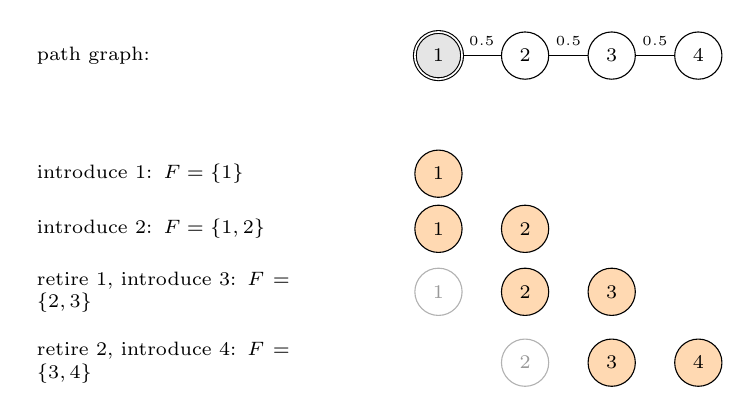
\begin{tikzpicture}[
  vtx/.style={draw, circle, minimum size=6mm, font=\scriptsize},
  seedv/.style={vtx, fill=gray!20, double},
  frontv/.style={vtx, fill=orange!30},
  retv/.style={vtx, fill=white, draw=black!30, text=black!40},
  steplab/.style={font=\scriptsize, align=left, text width=34mm}
]
\node[steplab] at (0,3.1) {path graph:};
\node[seedv] (g1) at (3.4,3.1) {$1$};
\node[vtx] (g2) at (4.5,3.1) {$2$};
\node[vtx] (g3) at (5.6,3.1) {$3$};
\node[vtx] (g4) at (6.7,3.1) {$4$};
\draw (g1) -- node[above, font=\tiny]{$0.5$} (g2);
\draw (g2) -- node[above, font=\tiny]{$0.5$} (g3);
\draw (g3) -- node[above, font=\tiny]{$0.5$} (g4);
\node[steplab] at (0,1.6) {introduce 1: $F=\{1\}$};
\node[steplab] at (0,0.9) {introduce 2: $F=\{1,2\}$};
\node[steplab] at (0,0.1) {retire 1, introduce 3: $F=\{2,3\}$};
\node[steplab] at (0,-0.8) {retire 2, introduce 4: $F=\{3,4\}$};
\node[frontv] at (3.4,1.6) {$1$};
\node[frontv] at (3.4,0.9) {$1$}; \node[frontv] at (4.5,0.9) {$2$};
\node[retv] at (3.4,0.1) {$1$}; \node[frontv] at (4.5,0.1) {$2$}; \node[frontv] at (5.6,0.1) {$3$};
\node[retv] at (4.5,-0.8) {$2$}; \node[frontv] at (5.6,-0.8) {$3$}; \node[frontv] at (6.7,-0.8) {$4$};
\end{tikzpicture}}
\caption{Frontier evolution of \texttt{ExactSpread} on the path example}
\label{fig:twig-path-example}
\end{subfigure}%
\hfill
\begin{subfigure}[t]{0.5\textwidth}
\centering
\resizebox{\linewidth}{!}{%
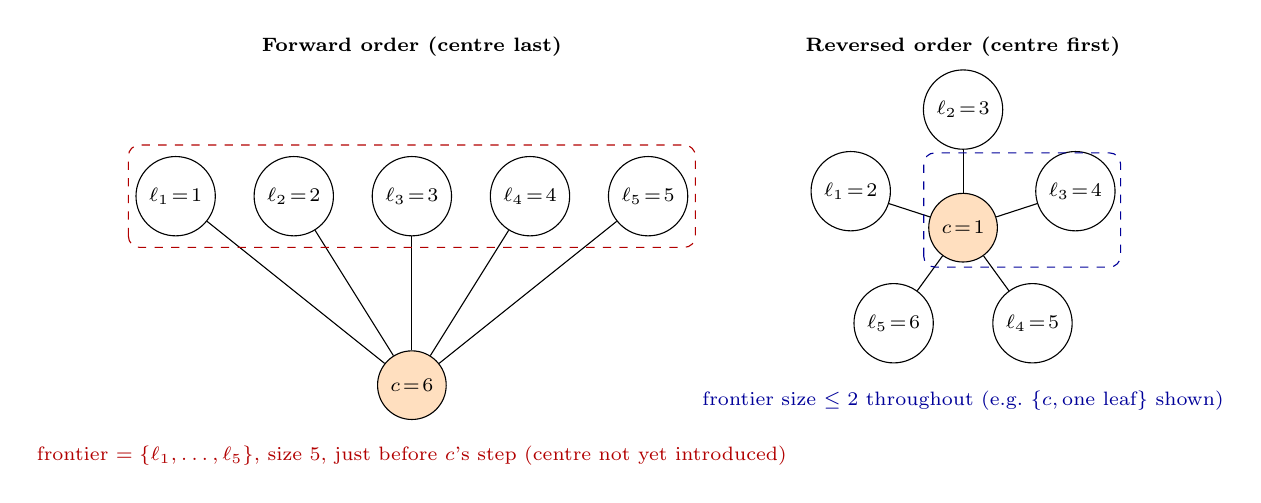
\begin{tikzpicture}[
  leaf/.style={draw, circle, fill=white, minimum size=6.5mm, font=\scriptsize},
  ctr/.style={draw, circle, fill=orange!25, minimum size=6.5mm, font=\scriptsize},
  lab/.style={font=\scriptsize, midway}
]
\begin{scope}
\node at (0,2.3) [font=\scriptsize\bfseries] {Forward order (centre last)};
\node[ctr] (c) at (0,-2) {$c\!=\!6$};
\foreach \k/\x in {1/-3,2/-1.5,3/0,4/1.5,5/3} {
  \node[leaf] (l\k) at (\x,0.4) {$\ell_\k\!=\!\k$};
  \draw (c) -- (l\k);
}
\draw[dashed, red!70!black, rounded corners] (-3.6,-0.25) rectangle (3.6,1.05);
\node[red!70!black, font=\scriptsize] at (0,-2.9) {frontier $=\{\ell_1,\dots,\ell_5\}$, size $5$, just before $c$'s step (centre not yet introduced)};
\end{scope}
\begin{scope}[xshift=7cm]
\node at (0,2.3) [font=\scriptsize\bfseries] {Reversed order (centre first)};
\node[ctr] (c2) at (0,0) {$c\!=\!1$};
\foreach \k/\ang/\ord in {1/162/2,2/90/3,3/18/4,4/-54/5,5/-126/6} {
  \node[leaf] (m\k) at (\ang:1.5) {$\ell_\k\!=\!\ord$};
  \draw (c2) -- (m\k);
}
\draw[dashed, blue!60!black, rounded corners] (-0.5,-0.5) rectangle (2.0,0.95);
\node[blue!60!black, font=\scriptsize] at (0,-2.2) {frontier size $\le2$ throughout (e.g.\ $\{c,\text{one leaf}\}$ shown)};
\end{scope}
\end{tikzpicture}}
\caption{Forward vs.\ reversed elimination order on $K_{1,5}$}
\label{fig:star-direction}
\end{subfigure}

\caption{Two elimination-order examples from Section~\ref{sec:twig}. (a) Orange = in the frontier $F$; grey outline = retired. The frontier
never exceeds size $2$: a path has treewidth $1$, and either
endpoint-to-endpoint order keeps only the just-retired vertex's successor
and the newly-introduced vertex active at once. Each orange configuration
branches on its live-edge outcome as in the text; Table~\ref{tab:twig-example}
lists all eight histories. (b) Left: centre processed last, so every leaf
is introduced but cannot retire until it arrives, growing the frontier to
all $5$ leaves. Right: centre processed first, so each leaf retires the
instant it is introduced and the frontier never exceeds $2$
(Proposition~\ref{prop:direction}).}
\end{figure}

\subsection{Empirical validation}\label{sec:twig-empirical}

Combining the collapse of Theorem~\ref{thm:twig-collapse} with the reversed
processing order of Proposition~\ref{prop:direction} makes exact evaluation
tractable on real, non-synthetic small networks:

\begin{table}[h]
\centering
\caption{Exact evaluation feasibility on real small networks\label{tab:twig-feasibility}}
\begin{tabular}{@{}lcccc@{}}
\hline
\up Network & $n$ & min-fill-in treewidth estimate & $w$ (reversed order, actually run) & \texttt{ExactSpreadFast.evaluate()} \\
\hline
\up Zachary karate club & 34 & 5 & 10 & 2.5 s \\
Iceland (sexual contact) & 75 & 4 & 12 & 51 s \\
\down Dolphin social network & 62 & $\sim$10 & 19 & infeasible (memory) \\
\hline
\end{tabular}
{\footnotesize The third column is the min-fill-in heuristic's estimate of the graph's
treewidth, used only to seed a good vertex \emph{order}. The fourth column,
$w=\max_i|F_i|-1$ (Section~\ref{sec:treewidth-prelim}), is the width
\texttt{ExactSpreadFast} actually realizes once that order is reversed
(Proposition~\ref{prop:direction}) and run -- the quantity
Propositions~\ref{prop:xp-space}--\ref{prop:fpt-space}'s complexity bounds
are stated in terms of, and a pathwidth-type parameter, not the treewidth
estimate in the third column: min-fill-in targets treewidth, and on none of
these three graphs does the best linear order come close to matching it.
The two columns need not agree, and here they differ by roughly $2$--$3\times$
on every network; Section~\ref{sec:twig-complexity} discusses why $w$, not
treewidth, is the parameter that actually bounds this algorithm's state
space, and how large that gap can be (Section~\ref{sec:twig-direction}).
Before both fixes (Theorem~\ref{thm:twig-collapse} and reversed processing
order), karate did not finish in 60 s and Iceland/Dolphin were not
attempted.}
\end{table}

On the karate club network (one seed, random independent-cascade
probabilities in $[0.05,0.4]$), \texttt{greedy\_exact} -- greedy selection
using \texttt{ExactSpreadFast} itself as the marginal-gain oracle, with zero
sampling noise -- selects node 2 at budget 1 (expected spread falls from the
unblocked value to 7.98) and adds node 1 at budget 2 (expected spread
5.51). \citet{xie2023} prove $\FF(\cdot)$ is not supermodular in $B$ under
the independent-cascade model, so greedy carries no $(1-1/e)$-style
guarantee for IMIN, and \citet{xie2024} further show IMIN is APX-hard;
consistent with both results, comparing \texttt{greedy\_exact} against
\texttt{brute\_force\_optimal\_block} on 60 small random instances
($n=6$--$14$, budget 1--4) finds greedy exactly optimal in 56 of 60 and
strictly suboptimal in 4, by up to 84.6\% relative excess spread in the
worst case (mean excess 2.2\% across all 60). This is, to our knowledge, the
first exact (not Monte-Carlo-confounded) measurement of how often and how
badly greedy departs from optimal IMIN selection.


\subsection{Complexity comparison}\label{sec:complexity-comparison}

Table~\ref{tab:complexity} collects the cost of the exact methods of this paper next to the sampling-based planners they are used to check, so the price of exactness can be read off in one place. TWIG's two variants solve a strictly harder problem than AG and GR (exact evaluation of $\FF(B)$ rather than an unbiased Monte Carlo estimate of it) and are not drop-in replacements for the sampling-based planners at the graph sizes those planners target. Proposition~\ref{prop:fpt-space}'s $n$-independence is what makes \texttt{ExactSpreadFast} usable compared with enumerating all $2^m$ live-edge realizations, but $B_{w+2}$ still grows very quickly in the width $w$ (Table~\ref{tab:bell-numbers}). \texttt{brute\_force\_optimal\_block} compounds TWIG's per-evaluation cost with an outer search over all size-$\le b$ subsets, which confines Section~\ref{sec:twig-empirical}'s optimality-gap study to $n\le14$. Removing the $(n+1)^{w+1}$ factor is also checked empirically: before the collapse of Theorem~\ref{thm:twig-collapse} and the reversed processing order of Proposition~\ref{prop:direction} were both applied, karate did not finish within 60 seconds under \texttt{ExactSpread}, whereas \texttt{ExactSpreadFast} evaluates it in 2.5 seconds.

\begin{table}[h]
\centering
\caption{Time complexity of the exact methods, with the sampling-based planners for reference.}\label{tab:complexity}
\small
\begin{tabular}{@{}ll@{}}
\hline
\up Method & Time complexity \\
\hline
\up AG \citep{xie2024} & $O(b\,\theta\,m\,\alpha(m,n))$ \\
GR \citep{xie2024} & $O(\min\{d^{out}_S,b\}\,\theta\,m\,\alpha(m,n))$ plus a replacement pass \\
\texttt{ExactSpread} (Proposition~\ref{prop:xp-space}) & one \texttt{evaluate}: $O(n\cdot B_{w+2}\cdot(n+1)^{w+1})$ (XP in $w$) \\
\texttt{ExactSpreadFast} (Proposition~\ref{prop:fpt-space}) & one \texttt{evaluate}: $O(n\cdot B_{w+2}\cdot\mathrm{poly}(w))$ (FPT in $w$) \\
\texttt{greedy\_exact} & $O(b)$ \texttt{evaluate} calls, each as above \\
\down \texttt{brute\_force\_optimal\_block} & $O(n^b)$ \texttt{evaluate} calls, each as above \\
\hline
\end{tabular}

\smallskip
{\footnotesize $\theta$: Monte Carlo sample size; $m$, $n$: edges and vertices of the region a planner processes; $\alpha$: inverse Ackermann function; $d^{out}_S$: out-degree of the seed set; $w$: width of the order actually run (Section~\ref{sec:treewidth-prelim}); $B_{w+2}$: the $(w+2)$-th Bell number.}
\end{table}

\begin{table}[h]
\centering
\caption{Bell numbers $B_{w+2}$, illustrating why the width $w$ (not just $n$) bounds \texttt{ExactSpreadFast}\label{tab:bell-numbers}}
\begin{tabular}{@{}lcccccccc@{}}
\hline
\up $w$ & 1 & 2 & 3 & 4 & 5 & 10 & 12 & 19 \\
\hline
\down $B_{w+2}$ & 5 & 15 & 52 & 203 & 877 & 4{,}213{,}597 & 190{,}899{,}322 & 474{,}869{,}816{,}156{,}751 \\
\hline
\end{tabular}
{\footnotesize $w$ ranges over the actually-realized widths in
Table~\ref{tab:twig-feasibility}'s fourth column (karate: $10$, iceland:
$12$, dolphin: $19$), not the smaller min-fill-in treewidth estimates in
its third column; the jump from $w=10$ to $w=19$ is the entire empirical
gap between ``tractable in seconds'' and ``infeasible by memory.''}
\end{table}
\section{Discussion and Limitations}\label{sec:discussion}

\subsection{When is TWIG the right tool?}\label{sec:discussion-twig}

TWIG is not a substitute for sampling-based evaluation at the sizes AG and GR target: Proposition~\ref{prop:fpt-space}'s $B_{w+2}$ state count is exponential in the width $w$ regardless of its independence of $n$, and Table~\ref{tab:twig-feasibility}'s real networks already span tractable (karate, $w=10$) to infeasible by memory (dolphin, $w=19$), two orders of magnitude below networks such as ca-GrQc in $n$ alone. Its role is as a validation instrument, certifying exactly how far greedy departs from optimal on small instances; greedy under noisy estimates is a source of bias that more sampling does not remove. Validating a greedy IMIN implementation against TWIG before trusting it at scale is analogous to unit-testing a numerical solver against closed-form instances. Three implementation bugs were caught only by exhaustive brute-force comparison, which shows why the check is not optional.

\subsection{Limitations}\label{sec:conclusion}

The optimality-gap study uses 60 random graphs with $n\le14$ and budgets up to $4$, so its percentages describe small instances; they are not an estimate of greedy's gap on large networks, where TWIG cannot run. The worst case of $84.6\%$ is the largest found among those 60, not a bound. Exact evaluation scales with the width realized by the vertex order, which can exceed the treewidth without bound on tree-like inputs and, as dolphin shows, can be too large on real networks of only a few dozen nodes. We did not compare TWIG's running time with that of \citet{nakamura2026}'s algorithm. 

\textbf{Code and data availability.} TWIG, \texttt{greedy\_exact}, \texttt{brute\_force\_optimal\_block} and the scripts for every experiment are released at \url{https://github.com/vinhqdang/trace_e}. The networks are the small public datasets cited in Section~\ref{sec:twig-empirical}.

\begin{thebibliography}{99}
\providecommand{\natexlab}[1]{#1}
\providecommand{\url}[1]{\texttt{#1}}
\providecommand{\urlprefix}{URL }

\bibitem[{Bodlaender(1988)}]{bodlaender1988}
Bodlaender HL (1988) Dynamic programming on graphs with bounded treewidth.
  \emph{Proc.\ 15th Internat.\ Colloquium on Automata, Languages and
  Programming (ICALP)}, 105--118.

\bibitem[{Budak et~al.(2011)Budak, Agrawal, and El~Abbadi}]{budak2011}
Budak C, Agrawal D, El~Abbadi A (2011) Limiting the spread of misinformation
  in social networks. \emph{Proc.\ 20th Internat.\ Conf.\ on World Wide Web
  (WWW)}, 665--674.

\bibitem[{Cygan et~al.(2015)Cygan, Fomin, Kowalik, Lokshtanov, Marx,
  Pilipczuk, Pilipczuk, and Saurabh}]{cygan2015}
Cygan M, Fomin FV, Kowalik {\L}, Lokshtanov D, Marx D, Pilipczuk M,
  Pilipczuk M, Saurabh S (2015) \emph{Parameterized Algorithms} (Springer,
  Cham).

\bibitem[{Fan et~al.(2013)}]{fan2013}
Fan L, Lu Z, Wu W, Thuraisingham B, Ma H, Bi Y (2013) Least cost rumor
  blocking in social networks. \emph{Proc.\ 33rd IEEE Internat.\ Conf.\ on
  Distributed Computing Systems (ICDCS)}, 540--549.

\bibitem[{He et~al.(2012)}]{he2012}
He X, Song G, Chen W, Jiang Q (2012) Influence blocking maximization in
  social networks under the competitive linear threshold model.
  \emph{Proc.\ 2012 SIAM Internat.\ Conf.\ on Data Mining (SDM)}, 463--474.

\bibitem[{Kempe et~al.(2003)Kempe, Kleinberg, and Tardos}]{kempe2003}
Kempe D, Kleinberg J, Tardos {\'E} (2003) Maximizing the spread of influence
  through a social network. \emph{Proc.\ 9th ACM SIGKDD Internat.\ Conf.\ on
  Knowledge Discovery and Data Mining (KDD)}, 137--146.

\bibitem[{Kinnersley(1992)}]{kinnersley1992}
Kinnersley NG (1992) The vertex separation number of a graph equals its
  path-width. \emph{Inform.\ Process.\ Lett.} 42(6):345--350.

\bibitem[{Maehara et~al.(2017)Maehara, Suzuki, and Ishihata}]{maehara2017}
Maehara T, Suzuki H, Ishihata M (2017) Exact computation of influence
  spread by binary decision diagrams. \emph{Proc.\ 26th Internat.\ Conf.\
  on World Wide Web (WWW)}, 947--956.

\bibitem[{Nakamura and Nishino(2026)}]{nakamura2026}
Nakamura K, Nishino M (2026) Linear-time exact computation of influence
  spread on bounded-pathwidth graphs. \emph{20th Scandinavian Sympos.\ on
  Algorithm Theory (SWAT)}, LIPIcs vol.\ 370, Article 34.

\bibitem[{Nguyen et~al.(2012)}]{nguyen2012}
Nguyen NP, Yan G, Thai MT, Eidenbenz S (2012) Containment of misinformation
  spread in online social networks. \emph{Proc.\ 4th Annual ACM Web Sci.\
  Conf.\ (WebSci)}, 213--222.

\bibitem[{Provan and Ball(1983)}]{provan1983}
Provan JS, Ball MO (1983) The complexity of counting cuts and of computing
  the probability that a graph is connected. \emph{SIAM J.\ Comput.}
  12(4):777--788.

\bibitem[{Valiant(1979)}]{valiant1979}
Valiant LG (1979) The complexity of enumeration and reliability problems.
  \emph{SIAM J.\ Comput.} 8(3):410--421.

\bibitem[{Wang et~al.(2013)Wang, Zhao, Chen, Li, Zhang, and Xia}]{wang2013blocking}
Wang S, Zhao X, Chen Y, Li Z, Zhang K, Xia J (2013) Negative influence
  minimizing by blocking nodes in social networks. \emph{Late-Breaking
  Developments in the Field of Artificial Intelligence, Papers Presented at
  the 27th AAAI Conf.\ on Artificial Intelligence}, AAAI Technical Report
  WS-13-17, 134--136.

\bibitem[{Wang et~al.(2024)Wang, Wu, Wang, Zhang, Qin, Zhang, and Lin}]{wang2024sandwich}
Wang J, Wu Y, Wang X, Zhang Y, Qin L, Zhang W, Lin X (2024) Efficient
  influence minimization via node blocking. \emph{Proc.\ VLDB Endowment}
  17(10):2501--2513.

\bibitem[{Xie et~al.(2023)Xie, Zhang, Wang, Lin, and Zhang}]{xie2023}
Xie J, Zhang F, Wang K, Lin X, Zhang W (2023) Minimizing the influence of
  misinformation via vertex blocking. \emph{Proc.\ 39th IEEE Internat.\
  Conf.\ on Data Engineering (ICDE)}, 3096--3108.

\bibitem[{Xie et~al.(2024)Xie, Zhang, Wang, Liu, Lin, and Zhang}]{xie2024}
Xie J, Zhang F, Wang K, Liu J, Lin X, Zhang W (2024) Influence minimization
  via blocking strategies. \emph{INFORMS J.\ Comput.}, forthcoming. Code:
  \texttt{github.com/INFORMSJoC/2024.0591}, arXiv:2312.17488.

\bibitem[{Zareie and Sakellariou(2021)}]{zareie2021}
Zareie A, Sakellariou R (2021) Minimizing the spread of misinformation in
  online social networks: A survey. \emph{J.\ Network and Computer
  Applications} 186:103094.

\end{thebibliography}

\appendix
\section{Proofs for Section~\ref{sec:twig}}\label{ec:twig-proofs}

\begin{repeatlemma}[Invariant maintained by \texttt{ExactSpread}]\label{ec:lem:invariant}
Fix $B$ and a step $i$. For every configuration $\kappa=(\Pi,\rho)$ with
$P_\kappa>0$ after step $i$,
\begin{align*}
P_\kappa=\Pr\nolimits_\omega\Bigl[\;&\Pi\text{ is the partition of }F_i\text{
by connectivity in }\bigl(F_i^{\ge},\,\omega|_{E_i}\bigr),\\
&\text{seed-containing part collapsed to SEED; and}\\
&\forall\text{ non-SEED block }b,\ \rho(b)=\bigl|
\{u:\mathrm{last}(u)\le i,\\
&\qquad u\text{ retired non-seed},\ u\sim_\omega b\}
\bigr|\;\Bigr],
\end{align*}
where $E_i$ is the set of edges processed by step $i$ (both endpoints
introduced, neither endpoint in $B$), $F_i^{\ge}=\{x\notin B:\mathrm{pos}(x)
\le i\}$ is every vertex introduced so far (active or already retired), and
$u\sim_\omega b$ means $u$ is connected, via live edges of $E_i$ within
$F_i^{\ge}$, to the current representative of block $b$. Moreover
$$\mathrm{acc}_i=\sum_{v\in V\setminus S\setminus B\,:\,\mathrm{last}(v)\le
i}\Pr\nolimits_\omega\bigl[v\sim_\omega\text{ some seed, using only edges of
}E_i\bigr].$$
\end{repeatlemma}
\begin{proof}
By induction on $i$. \emph{Base case} $i=-1$ (before any step): $F_{-1}
=\varnothing$, the unique configuration is the empty partition with $P=1$,
$\mathrm{acc}=0$, and both sides of the claimed identities are vacuously
true ($E_{-1}=\varnothing$, no vertex has retired).

\emph{Introduce.} Adding $v$ as a new singleton block changes nothing about
already-active vertices' connectivity (no new edge is realized), and
correctly starts $v$'s own block (SEED if $v\in S$, pending $0$ otherwise,
since $v$ is trivially connected to itself and, being newly introduced, to
nothing else yet). The invariant is preserved for $\Pi$ and, since no new
edges enter $E_i$, for $\mathrm{acc}$.

\emph{Process\_edge$(u,v)$.} This is the only place a new edge $(u,v)$
enters $E_i$. Conditioning on its two outcomes (independent of every other
edge's realization, by the independent-cascade model's edge independence)
exactly reproduces the two branches: tails leaves $\Pi$, $\rho$,
$\mathrm{acc}$ untouched, matching that $(u,v)\notin\omega$ leaves
connectivity and every retired vertex's membership unchanged. Heads merges
$u$'s and $v$'s blocks, which is exactly the effect of adding a live edge to
a union-find-style connectivity structure. If the merge is into SEED: every
already-retired vertex $u'$ counted in the merging block's $\rho(b)$ is, by
the outer induction hypothesis, connected (via $E_i\setminus\{(u,v)\}$) to
$b$'s current representative, hence now (with $(u,v)$ live) transitively
connected to a seed for the first time in this history -- exactly one unit
each is owed to $\mathrm{acc}$, contributing $p(u,v)\cdot\rho(b)$ in
expectation over this branch, matching the update; $\rho(b)$ is then
correctly discharged (those vertices will never need to be paid for again,
since a vertex is reached at most once). If the merge is between two
ordinary blocks, no vertex's fate is decided yet (neither is connected to a
seed), so $\mathrm{acc}$ is untouched and the two blocks' pending vertex
sets simply become one, i.e.\ $\rho(b_1)+\rho(b_2)$, matching the update.

\emph{Retire$(u)$.} $u$ retiring means $\mathrm{last}(u)=i$: every edge
incident to $u$ is already in $E_i$, so $u$'s connectivity to everything
else active or retired is already fully determined and will never change.
If $u$'s block is already SEED: $u$ is reached with probability $P_\kappa$
in this history, contributed to $\mathrm{acc}$ unless $u$ itself is a seed
(seeds are excluded from ``reached,'' matching the definition of
$\FF(B)$). Otherwise $u$'s fate is not yet decided; deferring it into
$\rho(b)$ is exactly the claimed count (one more retired vertex now
connected to $b$), \emph{unless} $b$ has no other active member, in which
case $b$ can never merge with anything else in the future (its only
remaining edges were already all processed, by definition of retirement
having emptied it of active representatives) -- correctly discharging
vertices that are provably never reached. Removing $u$ from $\Pi$ matches
$F_i\setminus\{u\}$.
\end{proof}

\begin{repeattheorem}[Theorem~\ref{thm:twig-correct} (Correctness of \texttt{ExactSpread})]
\texttt{ExactSpread}$(G,p,S)$.evaluate$(B)=\FF(B)$ for every $B$.
\end{repeattheorem}
\begin{proof}
Apply Lemma~\ref{ec:lem:invariant} at $i=n-1$ (the last step): $F_{n-1}
=\varnothing$ (every vertex has retired by the time all its neighbors,
which include itself, have been introduced), $E_{n-1}=E\setminus(B$-incident
edges$)$, i.e.\ all of $G_B$'s edges, and every non-seed, non-blocked
vertex has $\mathrm{last}(v)\le n-1$. The second identity of
Lemma~\ref{ec:lem:invariant} then reads $\mathrm{acc}_{n-1}=
\sum_{v\in V\setminus S\setminus B}\Pr_\omega[v\sim_\omega\text{ some seed
in }G_B]=\FF(B)$, which is exactly what \texttt{evaluate}$(B)$
returns.
\end{proof}

\begin{repeatproposition}[Proposition~\ref{prop:xp-space} (State space of \texttt{ExactSpread})]
A configuration's partition-plus-optional-SEED-designation component,
for a frontier of size $m\le w+1$, ranges over $B_{m+1}\le B_{w+2}$
possibilities, the $(w+2)$-th Bell number, independent of $n$: an
$m$-element set has $B_m$ (unmarked) partitions, and marking one block of a
given partition $\Pi$ as $\mathrm{SEED}$ -- or marking none -- gives
$\mathrm{blocks}(\Pi)+1$ distinct configurations from that one partition, so
summing over all partitions of the $m$-element frontier gives
$\sum_\Pi(\mathrm{blocks}(\Pi)+1)=B_{m+1}$ in total (the worked example of
Section~\ref{sec:twig-example} exhibits this directly: at $m=1$, the single
partition $\{\{2\}\}$ yields the two configurations ``$\{2\}$ ordinary'' and
``$\{2\}\equiv\mathrm{SEED}$,'' matching $B_2=2$). But each configuration's
pending vector has up to $w+1$ components, each ranging over
$\{0,\dots,n\}$, so the number of distinct configurations at any step is at
most $B_{w+2}\cdot(n+1)^{w+1}$.
\end{repeatproposition}

\begin{repeattheorem}[Theorem~\ref{thm:twig-collapse} (Correctness of the linear-aggregation collapse)]
Fix a partition shape $s$ and, at some step, let
$\mathcal K_s=\{(s,\rho):P_{(s,\rho)}>0\}$. Define the aggregates
$P_s=\sum_{(s,\rho)\in\mathcal K_s}P_{(s,\rho)}$ and
$W_b=\sum_{(s,\rho)\in\mathcal K_s}P_{(s,\rho)}\cdot\rho(b)$ for each
non-SEED block $b$ of $s$. Then $(P_s,\{W_b\})_s$ can be updated, at every
step, by the same four rules \texttt{ExactSpreadFast} implements, and this
update yields the identical sequence of \texttt{acc} increments as
\texttt{ExactSpread}, for every $B$.
\end{repeattheorem}
\begin{proof}
We check each of the (at most) four ways a step transforms a configuration
$(s,\rho)\mapsto(s',\rho')$ within a fixed edge-outcome branch (shape
transitions never depend on $\rho$, only on $s$ and, for
\texttt{process\_edge}, the branch); linearity of each in $\rho$ is then
all that is needed.

\emph{Introduce a new non-seed block $b_0$.} $\rho'(b_0)=0$,
$\rho'(b)=\rho(b)$ otherwise, $s'=s\cup\{b_0\}$ is independent of $\rho$.
Then $W'_{b_0}=\sum_\rho P_\rho\cdot 0=0$ and $W'_b=W_b$ for $b\ne b_0$: no
update needed for existing entries, new entry is (implicitly) $0$.

\emph{Process\_edge, tails.} $s'=s$, $\rho'=\rho$, but the whole branch
carries probability weight $(1-p_e)$: $P'_s=(1-p_e)P_s$ and
$W'_b=(1-p_e)W_b$ for every entry.

\emph{Process\_edge, heads, merge into SEED.} The payout added to
$\mathrm{acc}$ in this branch is
$p_e\sum_{(s,\rho)}P_\rho\cdot\rho(b)=p_e\cdot W_b$ exactly (a direct
algebraic identity, not a mean-field substitution). Block $b$ is then
dropped ($\rho'$ has no entry for it).

\emph{Process\_edge, heads, merge two ordinary blocks $b_1,b_2\to b$.}
$\rho'(b)=\rho(b_1)+\rho(b_2)$, so
$W'_b=\sum_\rho P_\rho(\rho(b_1)+\rho(b_2))=W_{b_1}+W_{b_2}$.

\emph{Retire, block still active.} $\rho'(b)=\rho(b)+1$ for the retiring
block, others unchanged: $W'_b=\sum_\rho P_\rho(\rho(b)+1)=W_b+P_s$ (using
the aggregate $P_s$, not a per-history increment).

\emph{Retire, block emptied.} $b$'s entry is dropped for every history in
$\mathcal K_s$ simultaneously (the condition ``no other active member''
depends only on $s$, not $\rho$), so $W'_b$ is simply omitted.

\emph{Retire, block is SEED, $u\notin S$.} $\mathrm{acc}$ gains
$\sum_\rho P_\rho=P_s$ in this branch.

Each case is an exact algebraic identity between the aggregate before and
the aggregate after, with no term dropped or approximated; by induction
over the sequence of steps, $(P_s,\{W_b\})$ computed by
\texttt{ExactSpreadFast} therefore equals the shape-lumped aggregate of
\texttt{ExactSpread}'s full distribution at every step, and in particular
produces the identical sequence of contributions to $\mathrm{acc}$.
\end{proof}

\begin{repeatproposition}[Proposition~\ref{prop:fpt-space} (State space of \texttt{ExactSpreadFast})]
The number of distinct states at any step is at most $B_{w+2}$ (one
$(P_s,\{W_b\})$ tuple per shape), independent of $n$.
\end{repeatproposition}

\begin{repeatproposition}[Proposition~\ref{prop:direction} (Star graphs separate forward and reversed elimination order)]
Let $T_k$ be the star $K_{1,k}$, $n=k+1$. Min-fill-in computes the
elimination order $\pi=(\ell_1,\dots,\ell_k,c)$, correctly certifying
treewidth $1$. Running the schedule of Section~\ref{sec:prelim} directly on
$\pi$ (the centre processed last) produces a frontier of size $k=n-1$
immediately before the centre's step. Running it on $\mathrm{reverse}(\pi)$
(the centre processed first) keeps the frontier at size at most $2$
throughout.
\end{repeatproposition}
\begin{proof}
Immediate from the definitions of Section~\ref{sec:prelim}: under $\pi$,
$\mathrm{last}(\ell_i)=\mathrm{pos}(c)=k$ for every leaf (its only neighbor
$c$ is introduced last), so no leaf retires before step $k$, giving
$F_{k-1}=\{\ell_1,\dots,\ell_k\}$; under $\mathrm{reverse}(\pi)$,
$\mathrm{last}(\ell_i)=\mathrm{pos}(\ell_i)$ (once $c$ is already active,
$\ell_i$'s only edge is processed the instant $\ell_i$ is introduced, and
$c$ is not $\ell_i$'s own last neighbor to be introduced -- it already was),
so every leaf retires the step after it is introduced, and $c$ itself
retires only at the final step (its own $\mathrm{last}$ is the position of
the last-introduced leaf), giving $|F_i|\le 2$ for all $i$.
\end{proof}

\section{Experimental Protocol}\label{ec:reproducibility}
Random small graphs, $n=6$--$14$, edge density such that the realized
width $w$ (Section~\ref{sec:treewidth-prelim}) stays at most 5--6, budget
1--4, one to four seeds. \texttt{greedy\_exact} and
\texttt{brute\_force\_optimal\_block} both run with the identical exact
oracle \texttt{ExactSpreadFast.evaluate}, so any discrepancy is a true
optimality gap, not sampling noise. 60 instances were drawn; the oracle's
correctness was independently checked by exhaustive summation over all
$2^{|E|}$ live-edge subsets on graphs up to $n=9$ (2000+ test cases for
\texttt{ExactSpread}, 1000+ for \texttt{ExactSpreadFast}), matching
Theorems~\ref{thm:twig-correct} and \ref{thm:twig-collapse}.

\end{document}
